\documentclass{article}

% Packages for mathematical symbols and equations
\usepackage{amsmath}
\usepackage{cancel}
\usepackage{amsthm}
\usepackage{amssymb}
\usepackage{bbm}
\usepackage{graphicx}
\graphicspath{ {./assets/} }
\usepackage[a4paper, total={18cm, 25cm}]{geometry}

% Title and author information
\title{Introduction To Sound Processing}
\author{Oded Vaalany 208230474}

\begin{document}

\maketitle

\section{Theoretical Part}
\subsection{Fourier Transform and Convlution}
Prove that $F[x_1(t)\cdot x_2(t)]= \frac{1}{2\pi} \big ( X^F_1(w)\ast X^F_2 (w)\big)$
\begin{proof}

lets donate $x_1:=f$ and $x_2:=g$ and $X^F_1(w):=F$ and $X^F_2(w):=G$ 
\newline
let recall that: 
\begin{itemize}
    \item $f(t) = FT^{-1}\big(F(\omega)\big) = \frac{1}{\sqrt{2\pi}}\int^{\infty}_{-\infty}F(\omega)e^{i2\pi \omega t}d \omega$
    \item $g(t) = FT^{-1}\big(G(\omega)\big) = \frac{1}{\sqrt{2\pi}}\int^{\infty}_{-\infty}G(\omega)e^{i2\pi \omega t}d \omega$
\end{itemize}

let's start by proving: $F(\omega -k) = F(\omega)\cdot e^{i2\pi k t} $
\newline
\begin{equation}
    \begin{aligned}
        F(\omega -k) & = \frac{1}{\sqrt{2\pi}}\int^{\infty}_{-\infty}f(t)e^{-i2\pi t(\omega -k)}dt\\
        & = \frac{1}{\sqrt{2\pi}}\int^{\infty}_{-\infty}f(t)e^{-i2\pi t\omega}e^{i2\pi t k}dt\\
        & = F(\omega)\cdot e^{i2\pi k t}
    \end{aligned}
\end{equation}
Now we can write the following:
\begin{equation}
    \begin{aligned}
        s(t) &= FT^{-1}\bigg[\frac{1}{2\pi}F(\omega) \ast G(\omega)\bigg](t)\\
        & = \frac{1}{2\pi}\int^\infty_{-\infty}\big(F(\omega)\ast G(\omega)\big)e^{i2\pi \omega t} d\omega\\
        & = \frac{1}{\sqrt{2\pi}}\int^\infty_{-\infty}\frac{1}{\sqrt{2\pi}}\bigg(\int^\infty_{-\infty}F(\omega-k)G(k) dk\bigg)e^{i2\pi \omega t} d\omega\\
        & = \frac{1}{\sqrt{2\pi}}\int^\infty_{-\infty}\frac{1}{\sqrt{2\pi}}\bigg(\int^\infty_{-\infty}F(\omega-k)G(k)\cdot e^{i2\pi \omega t} d\omega\bigg) dk\\
        & = \frac{1}{\sqrt{2\pi}}\int^\infty_{-\infty} G(k)\bigg(\int^\infty_{-\infty}\frac{1}{\sqrt{2\pi}}\cdot F(\omega-k)\cdot e^{i2\pi \omega t} d\omega\bigg) dk\\
        & = \frac{1}{\sqrt{2\pi}}\int^\infty_{-\infty} G(k)\bigg(\overbrace{\int^\infty_{-\infty}\frac{1}{\sqrt{2\pi}}\cdot F(\omega)\cdot e^{i2\pi \omega t}\cdot e^{i2\pi kt} d\omega}\bigg) dk\\
        & = \overbrace{\frac{1}{\sqrt{2\pi}}\int^\infty_{-\infty}  G(k) \cdot e^{i2\pi kt} dk} \cdot f(t) \\
        & = g(t) \cdot f(t)
    \end{aligned}
\end{equation}
and therefore we can conclude that: $FT[x_1(t)\cdot x_2(t)]= \frac{1}{2\pi} \big ( X^F_1(w)\ast X^F_2 (w)\big)$
\end{proof}

\subsection{Laying the ground for Nyquist’s sampling thm}
let's recall:
\begin{itemize}
    \item $x_d(t) = \sum^\infty_{n=-\infty}x(nT)\cdot \delta(t-nT)=x(t)\sum^\infty_{n=-\infty}\delta(t-nT)$ 
    \item $s_T(t) = \sum^\infty_{n=-\infty}\delta(t-nT)$ where $\delta(x) = \mathbbm{1}_{x=0}(x)$
    \item $X^F(\omega)= \int^\infty_{-\infty}x(t)e^{-i\omega t}dt $
    \item $S^F_T(\omega) = \frac{2\pi}{T} \sum_n \delta(\omega-\frac{2\pi n}{T})$
\end{itemize}
\subsubsection{Prove: $X^F_d(\omega) = \frac{1}{2\pi}\big(X^F(\omega) \ast S^F_T (\omega)\big)$}
\begin{proof}
    $ $\newline
    from section 1.1 we can conclude that: $FT(x(t) \cdot s_T(t)) = \frac{1}{2\pi}\big(X^F(\omega) \ast S^F_T (\omega)\big)$ 
    now all we have to do is to show that $x_d(t)=x(t)\cdot s_T(t)$ and this will prove the statement.
    $ $\newline
    as we got from the definition of $x_d(t)$ we can write: $x_d(t)= x(t) \sum^{\infty}_{n=-\infty} \delta(t-nT)$ and from the definition of $s_T(t)$ we can write: $s_T(t) = \sum^{\infty}_{n=-\infty} \delta(t-nT)$
    $ $\newline
    now we can write: $x_d(t)= x(t) \cdot s_T(t)$ 
    $ $\newline and therefore we can conclude that: $X^F_d(\omega) =FT[x_d(t)] = FT[x(t)\cdot s_T(t)] \frac{1}{2\pi}\big(X^F(\omega) \ast S^F_T (\omega)\big)$
\end{proof} 

\subsubsection{Prove: \[\sum_n \int^\infty_{-\infty} X^F(\tilde{\omega})\delta\bigg(\tilde{\omega}-\bigg(\omega-\frac{2\pi n}{T}\bigg)\bigg)d\tilde{\omega} = \sum_n X^F\bigg(\omega - \frac{2\pi n}{T}\bigg) \]}

\begin{proof}
    $ $\newline
    let's start by developing some known terms:
    \begin{equation}
        \begin{aligned}
            X_d^F(\omega) & = \frac{1}{2\pi}\big(X^F(\omega) \ast S^F_T (\omega)\big)\\
            & = \frac{1}{2\pi}\int_{-\infty}^{\infty}X^F(\omega-k)\cdot S^F_T(k) dk\\
            & = \frac{1}{\cancel{2\pi}}\int_{-\infty}^{\infty}\biggl(X^F(\omega-k)\cdot \frac{\cancel{2\pi}}{T}\sum_n \delta\big(k-\frac{2\pi n}{T}\big) \biggr)dk\\
            & = \frac{1}{T}\int_{-\infty}^{\infty}\biggl(X^F(\omega-k)\cdot\sum_n \delta\big(k-\frac{2\pi n}{T}\big) \biggr)dk\\
        \end{aligned}
    \end{equation}
    Integration effecive only when $\delta(k-\frac{2\pi n}{T})$ is not zero, and this is only when $k=\frac{2\pi n}{T}$, so we can write:
    \begin{equation}
        \begin{aligned}
            \begin{aligned}
                & = \frac{1}{T}\int_{-\infty}^{\infty}\biggl(X^F(\omega-k)\cdot\sum_n \delta\big(k-\frac{2\pi n}{T}\big) \biggr)dk\\
                & = \frac{1}{T}\sum_n \int_{-\infty}^{\infty}X^F(\omega-k)\cdot \delta\big(k-\frac{2\pi n}{T}\big) dk\\
                & = \frac{1}{T}\sum_n X^F\bigg(\omega - \frac{2\pi n}{T}\bigg)
            \end{aligned}
        \end{aligned}
    \end{equation}
    now since $\delta(x) = 0$ when $x \neq 0$ we can conclude that $\delta(x) = \delta(-x) (\star)$ and therefore we can develop $X_d^F(\omega)$ as follows:
    \begin{equation}
        \begin{aligned}
            X_d^F(\omega) & = \frac{1}{2\pi}\big(X^F(\omega) \ast S^F_T (\omega)\big)\\
            & = \frac{1}{2\pi}\int_{-\infty}^{\infty}X^F(\tilde{\omega})\cdot S^F_T(\omega-\tilde{\omega}) d\tilde{\omega}\\
            & = \frac{1}{\cancel{2\pi}}\int_{-\infty}^{\infty}\biggl(X^F(\tilde{\omega})\cdot \frac{\cancel{2\pi}}{T}\sum_n \delta\big(\omega-\tilde{\omega}-\frac{2\pi n}{T}\big) \biggr)d\tilde{\omega}\\
            \text{positive sums} & = \frac{1}{T}\sum_n \int_{-\infty}^{\infty}X^F(\tilde{\omega})\cdot \delta\bigg(\omega-\tilde{\omega}-\frac{2\pi n}{T}\bigg) d\tilde{\omega}\\
            \text{from } \star & = \frac{1}{T}\sum_n \int_{-\infty}^{\infty}X^F(\tilde{\omega})\cdot \delta\bigg(\tilde{\omega}-w+\frac{2\pi n}{T}\bigg) d\tilde{\omega}\\
            & = \frac{1}{T}\sum_n \int_{-\infty}^{\infty}X^F(\tilde{\omega})\cdot \delta\bigg(\tilde{\omega}-\bigg(w-\frac{2\pi n}{T}\bigg)\bigg) d\tilde{\omega}
        \end{aligned}
    \end{equation}

    therefore we can conclude that: $\sum_n \int^\infty_{-\infty} X^F(\tilde{\omega})\delta\bigg(\tilde{\omega}-\bigg(\omega-\frac{2\pi n}{T}\bigg)\bigg)d\tilde{\omega} = \sum_n X^F\bigg(\omega - \frac{2\pi n}{T}\bigg)$
\end{proof}

\subsubsection{Prove: $X_d^F(\omega)=\frac{1}{T}\sum^\infty_{n=-\infty}X^F(w - \frac{2\pi n}{T})$}
\begin{proof}
    already proved in section 1.2.2
    $ $\newline
    \begin{equation}
        \begin{aligned}
            X_d^F(\omega) & = \frac{1}{2\pi}\big(X^F(\omega) \ast S^F_T (\omega)\big)\\
            & = \frac{1}{2\pi}\int_{-\infty}^{\infty}X^F(\omega-k)\cdot S^F_T(k) dk\\
            & = \frac{1}{\cancel{2\pi}}\int_{-\infty}^{\infty}\biggl(X^F(\omega-k)\cdot \frac{\cancel{2\pi}}{T}\sum_n \delta\big(k-\frac{2\pi n}{T}\big) \biggr)dk\\
            & = \frac{1}{T}\int_{-\infty}^{\infty}\biggl(X^F(\omega-k)\cdot\sum_n \delta\big(k-\frac{2\pi n}{T}\big) \biggr)dk\\
        \end{aligned}
    \end{equation}
    Integration effecive only when $\delta(k-\frac{2\pi n}{T})$ is not zero, and this is only when $k=\frac{2\pi n}{T}$, so we can write:
    \begin{equation}
        \begin{aligned}
            \begin{aligned}
                & = \frac{1}{T}\int_{-\infty}^{\infty}\biggl(X^F(\omega-k)\cdot\sum_n \delta\big(k-\frac{2\pi n}{T}\big) \biggr)dk\\
                & = \frac{1}{T}\sum_n \int_{-\infty}^{\infty}X^F(\omega-k)\cdot \delta\big(k-\frac{2\pi n}{T}\big) dk\\
                & = \frac{1}{T}\sum_n X^F\bigg(\omega - \frac{2\pi n}{T}\bigg)
            \end{aligned}
        \end{aligned}
    \end{equation}
\end{proof}

\subsubsection{Bonus}
    We want's to prove that $f_s > 2f_{\max} \iff \forall x_d(t)$ and $\forall |\omega| \leq \omega_{\max} \Rightarrow X_d^F(\omega) = \frac{1}{T}X^F(\omega)$
    when $f_s= \frac1T$ and $f_{\max} = \frac{\omega_{\max}}{2\pi}$
    $ $\newline
    \begin{proof}[$\Leftarrow$]
        Assume that exists $f_s < 2\cdot f_{\max}$ s.t $\forall x_d(t)$ and $\forall |\omega| \leq \omega_{\max} \Rightarrow X_d^F(\omega) = \frac{1}{T}X^F(\omega)$ \\
        first we can conclude that 
        \begin{equation}
            f_s < 2\cdot f_{\max} \Rightarrow \frac{1}{T} < \frac{2\cdot \omega_{\max}}{2\pi} \Rightarrow \frac{1}{T} < \frac{\omega_{\max}}{\pi} \iff 1 < \frac{\omega_{\max}T}{\pi} \iff -1 > -\frac{\omega_{\max}T}{\pi}
            \end{equation}
        let's have $x_d(t)$ and choose $\omega=-\omega_{\max}$, we can write: (let's donate $\omega_{\max}=\omega'$)
        \begin{equation}
            \begin{aligned}
                 \frac{1}{T}X^F(-\omega') &= X_d^F(-\omega')\\
                 &= \frac{1}{T}\sum^\infty_{n=-\infty}X^F(-\omega' - \frac{2\pi n}{T})\\
                    &= \frac{1}{T}\sum^0_{n=-1}X^F(-\omega' - \frac{2\pi n}{T})\\
                    &= \frac{1}{T}\bigg(X^F(-\omega' - \frac{2\pi \cdot 0}{T}) + X^F(-\omega' - \frac{2\pi \cdot -1}{T})\bigg)\\
                    \cancel{\frac{1}{T}X^F(-\omega')} &= \frac{1}{T}\bigg(\cancel{X^F(-\omega')} + X^F(-\omega' + \frac{2\pi}{T})\bigg)\\
                    0 &= X^F(-\omega' + \frac{2\pi}{T})
            \end{aligned}
        \end{equation}
        and we assumed for all $|\omega| \leq \omega_{\max} \Rightarrow X^F(\omega)\ne 0$
        so we recieved a contradiction and therefore we can conclude that $f_s \geq 2\cdot f_{\max}$\\
        $ $\newline It is very simpale to prove that $f_s \ne 2 \cdot f_{\max}$, we can just choose $\omega = -\omega_{\max}$ and we will get the same contradiction.
        and therefore we can conclude that $f_s > 2\cdot f_{\max}$
    \end{proof}

    \begin{proof}[$\Rightarrow$]
        Assume that $f_s > 2\cdot f_{\max}$
        $ $\newline
        we can conclude:
        \begin{equation}
            f_s > 2\cdot f_{\max} \Rightarrow \frac{1}{T} > \frac{2\cdot \omega_{\max}}{2\pi} \Rightarrow \frac{1}{T} > \frac{\omega_{\max}}{\pi} \iff \frac{\pi}{T} > \omega_{\max} \iff -\omega_{\max} > -\frac{\pi}{T}
        \end{equation}
        let's have $x_d(t)$ and choose $\omega$ so $|\omega|\leq \omega_{\max}$, we can write: (let's donate $\omega_{\max}=\omega'$)
        fisrt we can conclude:
        \begin{equation}
            |\omega| \leq \omega' \iff -\omega' \leq \omega \leq \omega' \Rightarrow -\frac{\pi}{T} < \omega < \frac{\pi}{T}  \Rightarrow -1 < \frac{\omega T}{\pi} < 1
        \end{equation}
        now we want to find for which $n$ exists  $|\omega-\frac{2\pi n}{T}| \leq \omega'$
        \begin{equation}
            \omega -\frac{2\pi n}{T} \leq \omega' \iff  \frac{\omega T}{\pi} - \frac{\omega' T}{\pi} \leq 2n \Rightarrow -1 +1 \leq 2n \Rightarrow 0 \leq 2n \Rightarrow n \geq 0           
        \end{equation}
        \begin{equation}
            \omega -\frac{2\pi n}{T} \geq -\omega' \iff  \frac{\omega T}{\pi} + \frac{\omega' T}{\pi} \geq 2n \Rightarrow 1 \geq 2n \Rightarrow \frac{1}{2} \geq n \Rightarrow n \leq 0
        \end{equation}
        so we can conclude that $n=0$ and therefore we can write using section 1.2.3:
        \begin{equation}
            \begin{aligned}
                X_d^F(\omega) &= \frac{1}{T}\sum^\infty_{n=-\infty}X^F(\omega - \frac{2\pi n}{T})\\
                &= \frac{1}{T}X^F(\omega - \frac{2\pi \cdot 0}{T})\\
                &= \frac{1}{T}X^F(\omega)
            \end{aligned}
        \end{equation}
        as we want to prove.
        therefore we can conclude that $f_s > 2\cdot f_{\max} \Rightarrow \forall x_d(t)$ and $\forall |\omega| \leq \omega_{\max} \Rightarrow X_d^F(\omega) = \frac{1}{T}X^F(\omega)$
        \end{proof}
        \begin{proof}[Conclusion]
            by proving both directions we can conclude that\\ $f_s > 2\cdot f_{\max} \iff \forall x_d(t)$ and $\forall |\omega| \leq \omega_{\max} \Rightarrow X_d^F(\omega) = \frac{1}{T}X^F(\omega)$
            when $f_s= \frac1T$ and $f_{\max} = \frac{\omega_{\max}}{2\pi}$
        \end{proof}
\subsection{we are given $x(t)=\sin(2\pi \cdot 1000\cdot t)+\sin(2\pi \cdot 5000 \cdot t)$ we sample $x(t)$ with 8KHz what frequencies will be present in the sampled signal?}
\begin{proof}
    first we need to calculate the fourier transform of $x(t)$:
    \begin{equation}
        \begin{aligned}
            x(t) &= \sin(2\pi \cdot 1000\cdot t)+\sin(2\pi \cdot 5000 \cdot t)\\
            X^F(\omega) &= \int_{-\infty}^{\infty}x(t)e^{-i\omega t}dt\\
            &= \int_{-\infty}^{\infty}\sin(2\pi \cdot 1000\cdot t)e^{-i\omega t}dt + \int_{-\infty}^{\infty}\sin(2\pi \cdot 5000 \cdot t)e^{-i\omega t}dt\\
            &= \frac{\pi}{i}\bigg(\delta(\omega - 1000 \cdot 2\pi) - \delta(\omega + 1000 \cdot 2\pi)\bigg) + \frac{\pi}{i}\bigg(\delta(\omega - 5000\cdot 2\pi) - \delta(\omega + 5000\cdot 2\pi)\bigg)\\
        \end{aligned}
    \end{equation}
    by the sampling theorem we know that the frequencies that will be present in the sampled signal are: $f_s \pm f_0$ where $f_s$ is the sampling frequency and $f_0$ is the frequency of the signal.
    $ $\newline
    therefore the frequencies that will be present in the sampled signal are: 7KHz 1KHz 3KHz 5KHz
\end{proof}

\section{Practical Part}
\subsection{Time Stretching}
I encountered an issue when using the $\textbf{naive\_time\_stretch\_stft}$ function to
stretch the sound in the time domain. The output sounds incorrect when I try to
stretch the time with a factor of 0.8, as the voices sound higher than the
original. Similarly, when I stretch it with a factor of 1.2, the voices sound
lower. This can be explained by the fact that stretching the signal in the time
domain does not take into consideration the frequency dimensions, resulting in
a disruption of the harmonic structure of the sound and destroying the
frequencies.\\

However, when I stretch the signal with $\textbf{naive\_time\_stretch\_stft}$ in its
frequency domain, even though we play it faster and slower, since we didn't
break the harmonic structure of the frequencies, the signal sounds the same
with the same frequencies, just with a different rhythm.

\subsection{Self Checking}
\begin{proof}[]
    \centering
    \begin{tabular}{cccc}
        1KHz sine fft & 3KHz sine fft & 1KHz+3KHz sine fft\\
        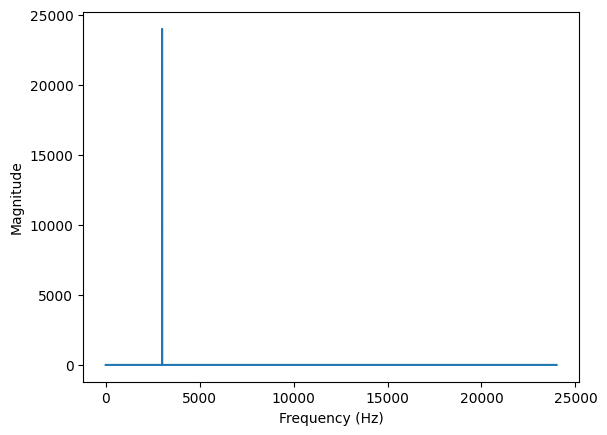
\includegraphics[width=.3\linewidth]{1kh_fft.png} & 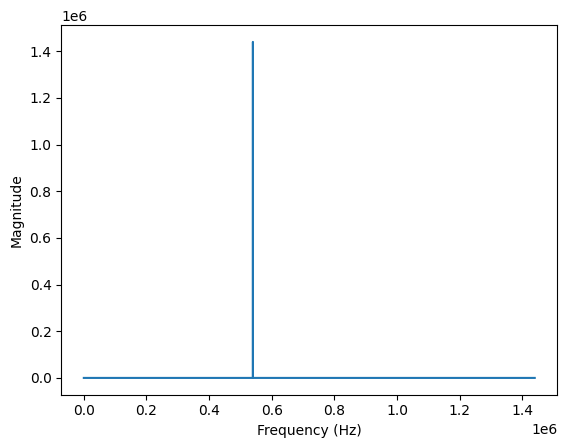
\includegraphics[width=.3\linewidth]{3kh_fft.png} & 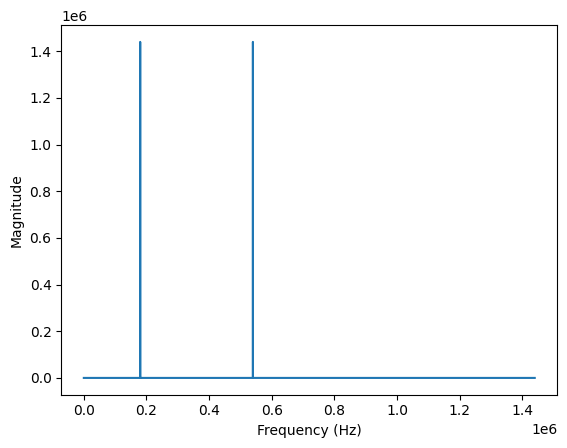
\includegraphics[width=.3\linewidth]{1kh+3kh_fft.png}
    \end{tabular}
\end{proof}

\subsection{Digit Classifier Pard B}
\begin{proof}[]
    here I will plot the FFT graph of the digit 1 and the digit 2 and the spectogram of the digits sounds.
    \centering
    \begin{tabular}{cccc}
        digit 1 fft & digit 2 fft\\
        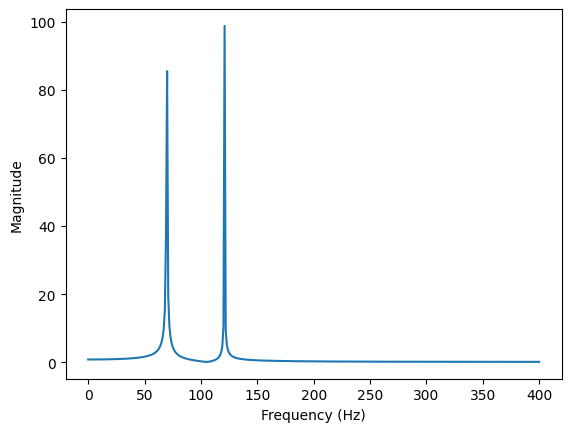
\includegraphics[width=.5\linewidth]{phone_1_fft.png} & 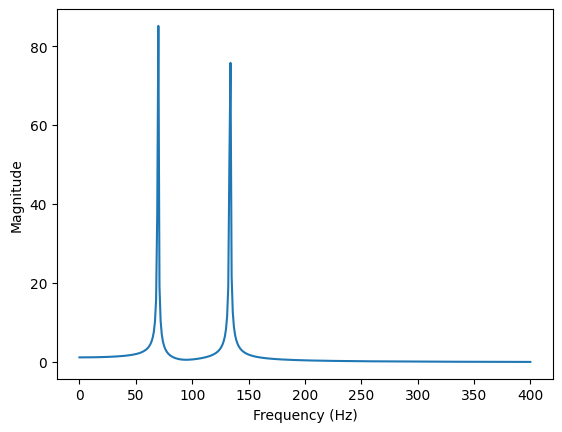
\includegraphics[width=.5\linewidth]{phone_2_fft.png}
    \end{tabular}
    spectogram\\
    \centering
        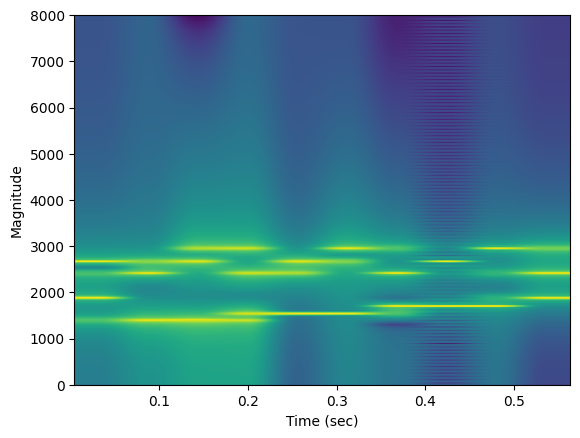
\includegraphics[width=.7\linewidth]{spect.png}
\end{proof}

\end{document}